% !TeX spellcheck = it_IT
\documentclass[10pt,a4paper]{article}

\usepackage[utf8]{inputenc}
\usepackage[T1]{fontenc}	
\usepackage[italian]{babel}
\usepackage{amsmath}
\usepackage{amsfonts}
\usepackage{amssymb}
\usepackage{graphicx}

\usepackage[left=2cm,right=2cm,top=2cm,bottom=2cm]{geometry}
\geometry{a4paper}

\usepackage{booktabs} % for much better looking tables
\usepackage{verbatim}
\usepackage{subfig} % make it possible to include more than one captioned figure/table in a single 

\usepackage{fancyhdr} % This should be set AFTER setting up the page geometry
\pagestyle{fancy} % options: empty , plain , fancy
\renewcommand{\headrulewidth}{0pt} % customise the layout...
\lhead{}\chead{}\rhead{}
\lfoot{}\cfoot{\thepage}\rfoot{}

%%% SECTION TITLE APPEARANCE
\usepackage{sectsty}
%\allsectionsfont{\sffamily\mdseries\upshape} % (See the fntguide.pdf for font help)
% (This matches ConTeXt defaults)

% pacchetti che mi fanno schifo ma uso lo stesso (Bob è scemo, ma anche Ale...)
\usepackage[cdot, thickqspace, squaren]{SIunits}
% il miglior pacchetto che potessi desiderare
\usepackage{float}
% macro che mi piacciono
\def\code#1{\texttt{#1}}


\title{Esercitazione 8: Oscillatore sinusoidale a ponte di Wien con OpAmp}

\author{Gruppo BE \\ Alessandro Candido, Roberto Ribatti}
\date{\today}
\begin{document}
\maketitle

\section{Scopo e strumentazione}
Lo scopo dell'esperienza è realizzare un oscillatore ad onda sinusoidale a ponte di Wien utilizzando un OpAmp.

\noindent La strumentazione usata è quella presente sul banco di lavoro, più l'OpAmp TL081 e due diodi.
%in realtà sia per l'OpAmp che per i diodi non abbiamo controllato che modello fossero, ce lo scriviamo comunque?
%c'è da inserire lo schema del circuito (si può anche copiare dalle slides)

\section{Loop gain del circuito}
Si è montato il circuito in \figurename{~\ref{circuito}} con i seguenti valori dei componenti:

\begin{figure}[H]
	\begin{minipage}{0.28\textwidth}
		\centering
		\begin{tabular}{l}
			$R_1 = \unit{9.95 \pm 0.9}{k\ohm}$ \\
			$R_2 = \unit{9.86 \pm 0.9}{k\ohm}$ \\
			$R_3 = \unit{9.73 \pm 0.9}{k\ohm}$ \\
			$R_4 = \unit{9.78 \pm 0.9}{k\ohm}$ \\
			$R_5 = \unit{9.84 \pm 0.9}{k\ohm}$ \\
			$C_1 = \unit{10.12 \pm 0.4}{\nano\farad}$ \\
			$C_1 = \unit{10.51 \pm 0.4}{\nano\farad}$ \\
			$POT_1 = \unit{10.15 \pm 0.9}{k\ohm}$ \\
		\end{tabular}
	\end{minipage}
	\begin{minipage}{0.75\textwidth}
		\centering
		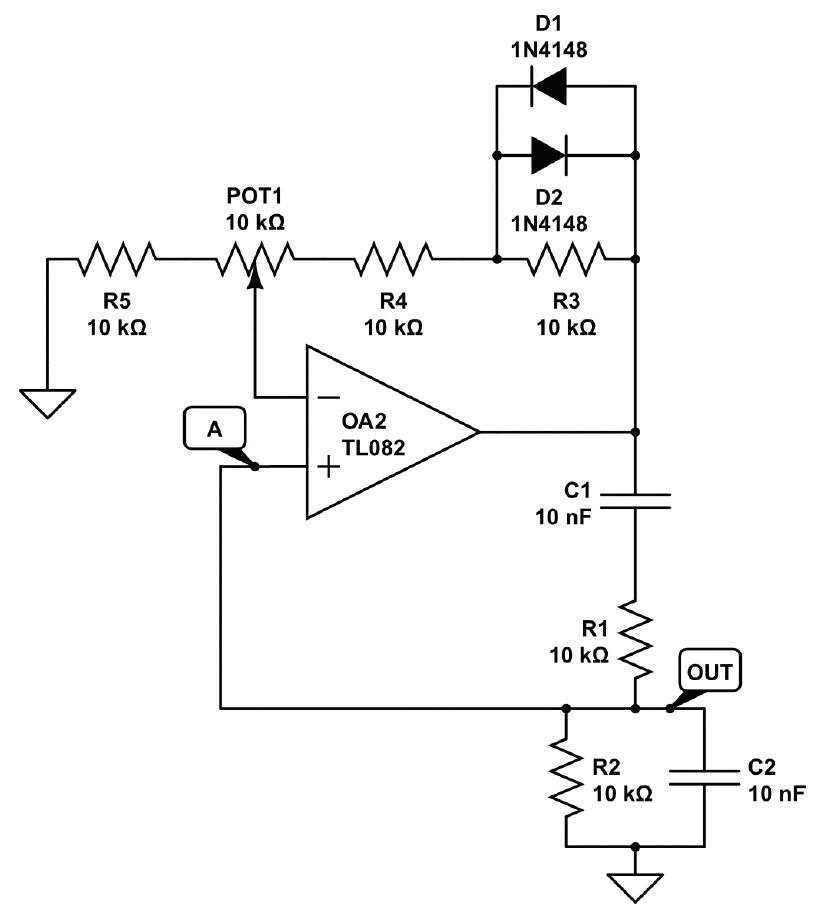
\includegraphics[width=0.6\textwidth]{../grafici/circuito.jpg}
		\caption{Circuito dell'oscillatore a ponte di Wien}
		\label{circuito}
	\end{minipage}
\end{figure}

Si è disconnesso il circuito nel punto A, connettendo l'ingresso non-invertente dell'OpAmp al generatore di funzioni e osservando con l'oscilloscopio il segnale all'altro estremo rimasto disconnesso.
Si è in questo modo misurato il loop gain (modulo e fase) per varie frequenze immesse dal generatore di funzioni ad un fisso valore della posizione del potenziometro. I dati raccolti sono riportati in appendice in (\tablename{~\ref{tab:loop}}).

Il loop gain atteso sarà il prodotto del guadagno $A$ del'OpAmp con la sua rete di feedback ($R_3$, $R_4$, $R_5$, $POT_1$ e i due diodi) e del guadagno $\beta$ della rete di reazione positiva ($C_1$, $R_1$, $C_2$ e $R_2$).

Fissati i valori delle resistenze $A$ dipenderà dalla tensione in input (dal cui valore dipenderà la resistenza dinamica dei diodi) e dalla posizione del potenziometro. La reazione $\beta$ dipenderà invece dalla frequenza secondo la seguente formula\footnote{nell'ipotesi che i prodotti $R_1 C_1$, $R_2  C_2$ e $R_2  C_1$ siano uguali, ipotesi in ottima approssimazione valida nel nostro caso.}:
\begin{equation*}
\beta = \frac{jf}{1-f^2+3jf}
\end{equation*}

Dove $f$ è espresso in unità di $f_0 = R_1C_1 \simeq R_2C_2 \simeq R_2C_1$. Segue che il modulo e la fase della rete di reazione saranno (con le stesse unità per $f$):
\begin{equation}
|\beta|=\frac{f}{f^4+7f^2+1}\hspace{2cm}\phi_{\beta} = \text{arctan} \biggl( \frac{1-f^2}{3f} \biggr)
\label{eq:beta}
\end{equation}

Con queste formule, moltiplicate per il guadagno costante $A$, si sono fittate le misure prese dei moduli e delle fasi del loop gain. I risultati ottenuti e i grafici dei fit sono riportati di seguito.
\begin{figure}[H]
	\begin{minipage}{0.2\textwidth}
		\begin{tabular}{l}
			$f_0^1 = \unit{1596 \pm 10}{\hertz}$ \\
			$|A| = 2.953 \pm 0.005$\\
			$corr(f_0,|A|) = 0.17$\\
			$\chi^2 /\text{ndof} = 16.5 / 13 $\\
			$p_{val} = 0.22$
		\end{tabular}
	\end{minipage}
	\begin{minipage}{0.8\textwidth}
		\centering
		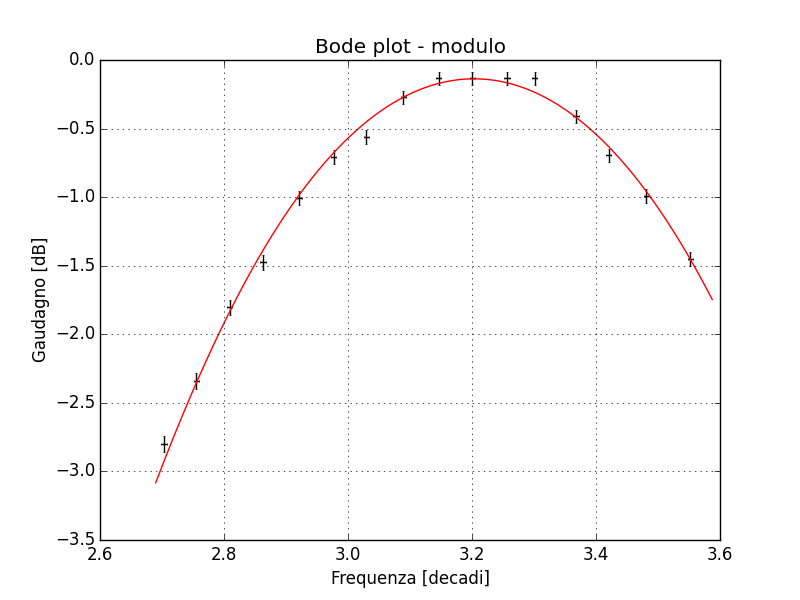
\includegraphics[width=0.95\textwidth]{../grafici/fit_loopgain_modulo.pdf}
		\caption{Dati e fit del modulo del guadagno di loop}
		\label{fig:Bode}
	\end{minipage}
\end{figure}

\begin{figure}[H]
	\begin{minipage}{0.2\textwidth}
		\begin{tabular}{l}
			$f_0^2 = \unit{1856 \pm 9}{\hertz}$ \\
			$\chi^2 /\text{ndof} = 23.1 / 14 $\\
			$p_{val} = 0.06$
		\end{tabular}
	\end{minipage}
	\begin{minipage}{0.8\textwidth}
		\centering
		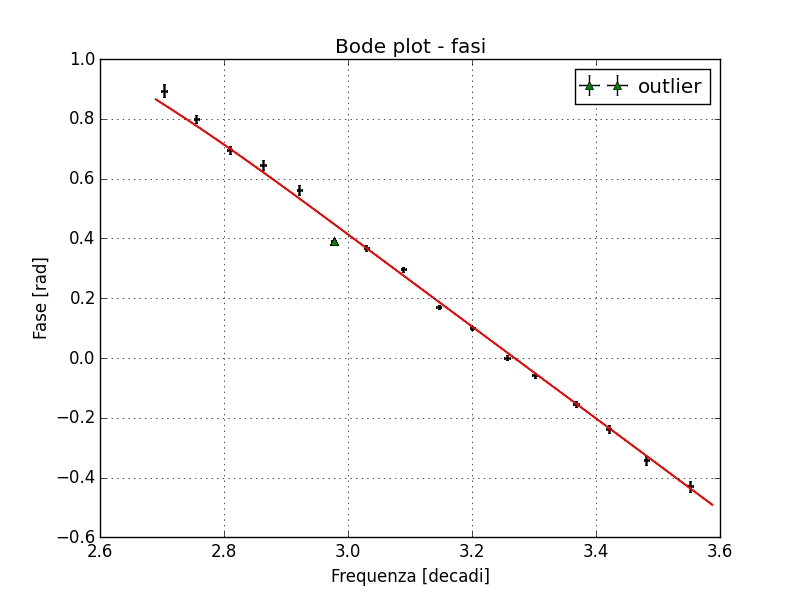
\includegraphics[width=0.95\textwidth]{../grafici/fit_loopgain_fase.pdf}
		\caption{Dati e fit della fase del loop}
		\label{fig:Bode}
	\end{minipage}
\end{figure}

%inserire risultati dei fit, quando si è capito quali sono quelli giusti

La frequenza a cui lo sfasamento si annulla è stata misurata e il valore è $f_0^3 = \unit{1.80 \pm 0.05}{\kilo\hertz}$.

Il valore atteso dalla teoria per $f_0$ è pari a $RC$ nell'ipotesi che i prodotti $R_1 C_1$, $R_2  C_2$ e $R_2  C_1$ siano uguali. 

In questo caso si ha: $1/(2\pi R_1 C_1) = \unit{1.58 \pm 0.06}{k\hertz}$, $1/(2\pi R_2 C_2) = \unit{1.54 \pm 0.06}{k\hertz}$ e $1/(2\pi R_2 C_1) = \unit{1.60 \pm 0.07}{k\hertz}$, per cui l'approssimazione è valida e posso considerare un valore atteso medio $f_0^{exp} = \unit{1.57 \pm 0.05}{k\hertz}$.

Questo valore atteso è compatibile con la frequenza ottenuta dal fit dei moduli, ma non con quella ottenuta dal fit delle fasi che a sua volta invece è compatibile con la frequenza misurata a cui la fase è nulla.\\

Si è osservato che l'ampiezza del segnale di output dipende in modo monotono dalla posizione del potenziometro. Questo è coerente con il comportamento atteso:
\begin{equation}
A = 1 + \frac{(1-\eta)POT_1 + R_4 + (R_3//R_{diodi})}{R_5 + \eta POT_1}
\label{eq:pot}
\end{equation}

In cui $c$ è la frazione di potenziometro che va verso $R_5$.

\section{Risposta in funzione della posizione del potenziometro}
Si è riconnesso il circuito nel punto A e si è osservata la dipendenza del segnale in uscita in funzione della posizione del potenziometro.

Si è ottenuto che per alti valori di $\eta$ non si osservava alcuna oscillazione, mentre al diminuire di $\eta$ (definito in \eqref{eq:pot}) l'ampiezza del segnale in output aumentava, fino a raggiungere la saturazione.

Questo comportamento trova riscontro con quanto atteso: infatti la condizione di Barkhausen impone come conseguenza che $A = 3$. Per ottenere questo valore dato un certo $\eta$ quello che varia è la resistenza dinamica dei diodi, e quindi il punto di lavoro.

Per cui, imponendo che $R = R_3 = R_4 = R_5 = POT_1 = \unit{10}{\kilo\ohm}$ e chiamondo $R_d$ la resistenza dinamica dei diodi, si ottiene dalla \eqref{eq:pot}:
\begin{equation}
A = 1 + \frac{2 - \eta + R//R_d}{1+\eta}
\end{equation}

Per cui per avere $A = 3$ con $\eta \sim 1$ si dovrebbe avere $(1 + R/R_{d})^{-1} \sim 3$, che è impossibile poiché il primo membro è sempre $\leq 1$.
Per $\eta$ più piccoli si riduce il valore richiesto per $(1 + R/R_{d})^{-1}$, infatti per $\eta = 1/3$ si ottiene che $(1 + R/R_{d})^{-1} = 1$, e questo è possibile per valori di $R_{d}$ molto elevati. Man mano che decresce $\eta$ decresce dunque il valore richiesto della resistenza dinamica, spostando il punto di lavoro a tensioni di output maggiori, fino ad arrivare a $\eta = 0 \implies (1 + R/R_{d})^{-1} = 0 \implies R_{d} = 0$ per cui uno dei diodi deve essere completamente in conduzione.

Per valori così piccoli di $\eta$ si porta l'output a saturazione portando alla distorsione delle onde sinusoidali come mostrato nell'immagine a destra in \figurename{~\ref{fig:dippot}}. Nell'immagine a sinistra è invece mostrato il funzionamento in regime lineare, per cui l'uscita è una sinusoide.

\begin{figure}[H]
    \centering
    \begin{minipage}{0.49\textwidth}
	    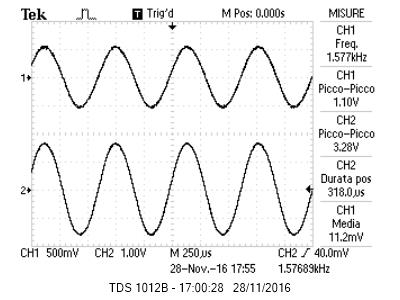
\includegraphics[width=\textwidth]{../oscilloscopio/punto2.jpg}
    \end{minipage}
    \begin{minipage}{0.49\textwidth}
        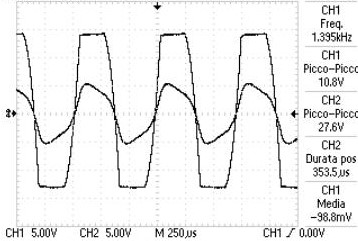
\includegraphics[width=\textwidth]{../oscilloscopio/punto5(scazzo).jpg}
    \end{minipage}
    \caption{Dipendenza del segnale in uscita dalla posizione del potenziometro}
    \label{fig:dippot}
\end{figure}

\section{Frequenza di oscillazione}
La frequenza di oscillazione misurata è pari a $\unit{1.57 \pm 0.02}{\kilo\hertz}$, compatibile con il valore teorico atteso $f_0^{exp}$ e con il valore ottenuto dal fit del modulo del guadagno.
% in questa sezione manca il confronto con la teoria, te lo lascio.

La frequenza di oscillazione osservata è risultata indipendente dalla posizione del potenziometro come del resto ci si aspettava poichè la posizione del potenziometro modifica il valore di $A$ ma non aggiunge una fase. La frequenza di oscillazione dipenderà solo dalla rete di reazione come visto nella formula della fase di $\beta$ in eq. \eqref{eq:beta}.

La frequenza di oscillazione risulta indipendente dalla tensione di alimentazione, fintanto che questa non diventi abbastanza ridotta da portare il segnale di output in clipping come mostrato in \figurename{~\ref{clipping}}.

\begin{figure}[H]
	\centering
	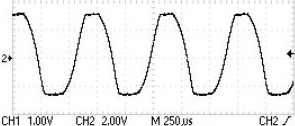
\includegraphics[width=0.4\textwidth]{../oscilloscopio/punto3(clipall)}
	\caption{Clipping dovuto alle basse tensioni di alimentazione dell'OpAmp}
	\label{clipping}
\end{figure}

\section{Guadagno all'innesco dell'oscillazione}

Ci si è posti alla posizione del potenziometro corrispondente all'innesco dell'oscillazione e si sono misurati i seguenti valori per le tensioni:

\begin{table}[H]
	\centering
	\begin{tabular}{cc}
        $ V_+ = \unit{256 \pm 8}{\milli\volt}$  & $V_{out} = \unit{820 \pm 26}{\milli\volt}$
	\end{tabular}
\end{table}

Da cui si ricava un guadagno $A = 3.20 \pm 0.14$ che è compatibile con 3 a poco più di $1\sigma$.

\section{Scopo dei diodi}
Lo scopo dei diodi è di inserire un elemento non lineare nella rete di amplificazione, in modo da stabilizzare la tensione sull'output.

Infatti se il potenziometro viene ruotato il guadagno $A$ cambia, e in risposta cambia il punto di lavoro dei diodi, impedendo al guadagno di modificarsi eccessivamente.

In particolare, con riferimento all'equazione \eqref{eq:pot}:
\begin{description}
\item[aumenta $\eta$] diminuirebbe il guadagno $A$ e la resistenza dinamica dei diodi tenderebbe ad aumentare, mantenendo quindi $A$ alto;
\item[diminuisce $\eta$] aumenterebbe il guadagno $A$ e i diodi andrebbero sempre più in conduzione, diminuendo quindi il guadagno $A$, cioè stabilizzandolo.
\end{description}

I diodi quindi svolgono il ruolo di feedback negativo sul guadagno $A$, cioè lo mantengono stabile rispetto alle variazioni di altri elementi, rendendo quindi possibile lavorare in regime lineare con un intervallo maggiore di valori.

In assenza di diodi, invece, si perde stabilità, e provando a ruotare il potenziometro si passa da un regime in cui non vi sono oscillazioni a un regime in cui le oscillazioni vanno in saturazione. Quest'ultimo regime è mostrato in \figurename{~\ref{fig:wdiod}}.

\begin{figure}[H]
    	\centering
        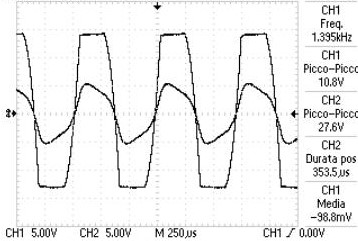
\includegraphics[width=0.5\textwidth]{../oscilloscopio/punto5(scazzo).jpg}
    \caption{Risposta del circuito in assenza di diodi}
    \label{fig:wdiod}
\end{figure}

\pagebreak
\section{Appendice: Dati acquisiti}
Si riportano qui le tabelle dei dati usati per i fit e i grafici.

\begin{figure}[H]
	\centering
	\resizebox{0.7\textwidth}{!}{
	\input{../tabelle/tab_loopgain1.txt}}
	\captionof{table}{Dati raccolti di modulo e fase del loop gain}
	\label{tab:loop}
\end{figure}

\end{document}
